
\documentclass[11pt,a4paper]{exam}
\usepackage[utf8]{inputenc}
\usepackage{graphicx, wrapfig}
\usepackage{subcaption}
\usepackage{amsmath}
\usepackage{amsthm}
\usepackage{amssymb}
\usepackage{mathtools}
\usepackage[shortlabels]{enumitem}

\renewcommand*{\proofname}{Prova}
% bold math
\usepackage{amsbsy}

% draw pictures (and graphs)
\usepackage{tikz}

% \usepackage[usenames,dvipsnames,svgnames,table]{xcolor}

% code in latex
\definecolor{dkgreen}{rgb}{0,0.6,0}
\definecolor{gray}{rgb}{0.5,0.5,0.5}
\definecolor{mauve}{rgb}{0.58,0,0.82}
\definecolor{newink}{rgb}{0,0.1,0.25}
\usepackage{caption}
\usepackage{listings}
\lstset{frame=tb,
  language=Python,
  aboveskip=3mm,
  belowskip=3mm,
  showstringspaces=false,
  columns=flexible,
  basicstyle={\small\ttfamily},
  numbers=none,
  numberstyle=\tiny\color{gray},
  keywordstyle=\color{blue},
  commentstyle=\color{dkgreen},
  stringstyle=\color{mauve},
  breaklines=true,
  breakatwhitespace=true,
  tabsize=3
}


\usepackage{multirow}

% definition equal
\newcommand\eqdef{\mathrel{\overset{\makebox[0pt]{\mbox{\normalfont\tiny\sffamily def}}}{=}}}

% independence equal
\newcommand\eqindep{\mathrel{\overset{\makebox[0pt]{\mbox{\normalfont\tiny\sffamily indep}}}{=}}}


% independent and identically distributed equal
\newcommand\eqiid{\mathrel{\overset{\makebox[0pt]{\mbox{\normalfont\tiny\sffamily i.i.d.}}}{=}}}

% * to cdot
% \mathcode`\*="8000
% {\catcode`\*\active\gdef*{\cdot}}
\usepackage[table,xcdraw]{xcolor}
% pseudo-code
\usepackage[portuguese, linesnumbered]{algorithm2e}
\newcommand\Recebe{\leftarrow}
\newcommand\Comment{\vartriangleright}
\SetKw{Devolva}{devolva}
% Example:
% \paragraph{}
% \SetAlgoNoLine
% \textsc{Título-Do-Algoritmo}($A, n$)\\
% \begin{algorithm}[H]
%   \Devolva $A$
% \end{algorithm}
%

% pair ceil
\DeclarePairedDelimiter{\ceil}{\lceil}{\rceil}

% pair ceil
\DeclarePairedDelimiter{\floor}{\lfloor}{\rfloor}

% images
\usepackage{graphicx}
\graphicspath{ {./} }
% use: \includegraphics[scale=1]{image}
\usepackage{float}

\setlength{\parindent}{3em}
\setlength{\parskip}{0.5em}

\usetikzlibrary{graphs,graphs.standard}

\newcount\nodecount
\tikzgraphsset{
  declare={subgraph N}%
  {
    [/utils/exec={\global\nodecount=0}]
    \foreach \nodetext in \tikzgraphV
    {  [/utils/exec={\global\advance\nodecount by1}, 
      parse/.expand once={\the\nodecount/\nodetext}] }
  },
  declare={subgraph C}%
  {
    [cycle, /utils/exec={\global\nodecount=0}]
    \foreach \nodetext in \tikzgraphV
    {  [/utils/exec={\global\advance\nodecount by1}, 
      parse/.expand once={\the\nodecount/\nodetext}] }
  }
}
\linespread{1.2}

\title{
    \textbf{Uma explicação sobre as características do grafo de Petersen}\\
    \large Bacharelado em Ciência da Computação\\
    MAC0320 - Introdução à Teoria dos Grafos
}
\author{Rogério Marcos Fernandes Neto\\
     NUSP: 10284632
}
\date{}
\begin{document}

\maketitle
\section{Introdução}
\par Quando se inicia o estudo sobre um grafos, são estudadas diversas
definições e características básicas que podemos quantificar ou atribuir
a eles. Um grafo interessante que aparece em meio a esse estudo é o
\textbf{grafo de Petersen}. O grafo de Petersen é um grafo bem
característico que pode ser definido da seguinte forma:
\paragraph{Definição 1:} Seja $X := \{1,2,3,4,5\}$.
O grafo de Petersen é o grafo $G=(V,A)$ onde $V=\{\{v,w\}:y,w,\in X,y \neq w\}$ e
$A:=\{\{u,v\}:u\cap v = \emptyset\}$

Existem várias representações possíveis vindas dessa definição. A mais
famosa é a seguinte figura:
\begin{figure}[H]
    \centering
    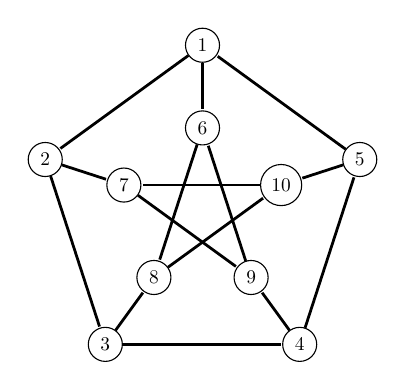
\begin{tikzpicture}[shorten >=0.5pt, auto, 
        every node/.style={scale=0.7}, scale=0.7]
        \tikzstyle{nodeStyle} = [circle,draw=black,fill=white]
        \tikzstyle{blackEdge} = [draw=black, line width=1]
        \node[nodeStyle] (V) at (90:1.5) {6};
        \node[nodeStyle] (A) at (90:3) {1};
        \node[nodeStyle] (W) at (162:1.5) {7};
        \node[nodeStyle] (B) at (162:3) {2};
        \node[nodeStyle] (X) at (234:1.5) {8};
        \node[nodeStyle] (C) at (234:3) {3};
        \node[nodeStyle] (Y) at (306:1.5) {9};
        \node[nodeStyle] (D) at (306:3) {4};
        \node[nodeStyle] (Z) at (378:1.5) {10};
        \node[nodeStyle] (E) at (378:3) {5};
        \path[blackEdge] (A) edge (B);
        \path[blackEdge] (B) edge (C);
        \path[blackEdge] (C) edge (D);
        \path[blackEdge] (D) edge (E);
        \path[blackEdge] (E) edge (A);
        \path[blackEdge] (A) edge (V);
        \path[blackEdge] (B) edge (W);
        \path[blackEdge] (C) edge (X);
        \path[blackEdge] (D) edge (Y);
        \path[blackEdge] (E) edge (Z);
        \path[blackEdge] (V) edge (X);
        \path[blackEdge] (X) edge (Z);
        \path[blackEdge] (Z) edge (W);
        \path[blackEdge] (W) edge (Y);
        \path[blackEdge] (Y) edge (V);
    \end{tikzpicture}
    \caption{Grafo de Petersen}
\end{figure}

As próximas seções são dedicados a explicar algumas características
desse grafo. Cada seção será inspirada em um capítulo apresentado pela
professora Yoshiko Wakabayashi. Não nos preocuparemos aqui em refazer
todas as definições apresentadas em aula mas sim aplica-las diretamente.
A menos que específicado de outra forma, iremos supor que o grafo $G$
referido nas notações matemáticas se referem ao grafo de Petersen

\section{Conceitos e Resultados Básicos}
O grafo de Petersen possui 10 vértices no total e 15 arestas, isso é,
$|V(G)| = 10$ e $|A(G)| = 15$. Além disso, esse grafo é \textbf{simples} e
\textbf{conexo}.  Todos os vértices do grafo de Petersen
possuem grau 3, isso pode ser conferido na \textbf{Figura 1}. Tal fato o
classfica como o grafo \textbf{$3$-regular}.
\par Como o grafo de Petersen possui 15, arestas, então seu grafo
complementar $\bar{G}$ posssui $|V(\bar{G})|=|V(G)|(|V(G)|-1)/2 -15 = 30$ arestas e deve ser um
grafo $6$-regular. Pelo número de arestas de $\bar{G}$ ja é possível
descartar a possíbilidade de $G$ ser \textbf{auto-complementar}. Uma possível
representação de $\bar{G}$ é:
\begin{figure}[H]
    \centering
    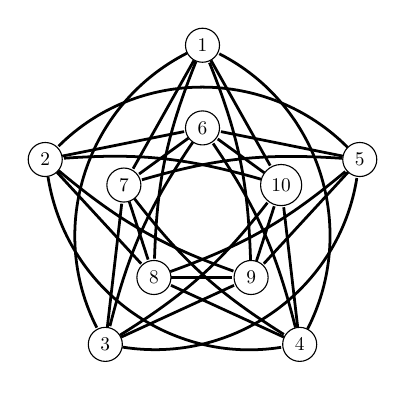
\begin{tikzpicture}[shorten >=0.5pt, auto,
        every node/.style={scale=0.7}, scale=0.7]
        \tikzstyle{nodeStyle} = [circle,draw=black,fill=white]
        \tikzstyle{blackEdge} = [draw=black, line width=1]
        \node[nodeStyle] (6) at (90:1.5) {6};
        \node[nodeStyle] (1) at (90:3) {1};
        \node[nodeStyle] (7) at (162:1.5) {7};
        \node[nodeStyle] (2) at (162:3) {2};
        \node[nodeStyle] (8) at (234:1.5) {8};
        \node[nodeStyle] (3) at (234:3) {3};
        \node[nodeStyle] (9) at (306:1.5) {9};
        \node[nodeStyle] (4) at (306:3) {4};
        \node[nodeStyle] (10) at (378:1.5) {10};
        \node[nodeStyle] (5) at (378:3) {5};
        \foreach \from/\to in {1/7, 1/10, 2/6, 2/8, 3/7, 3/9, 4/8, 4/10,
                                5/9, 5/6}
            \path[blackEdge] (\from) edge (\to);
        \foreach \from/\to in {5/2, 2/4, 4/1, 1/3, 3/5}
            \path[blackEdge] (\from) edge[bend right=45] (\to);
        \foreach \from/\to in {5/7, 7/4, 4/6, 6/3, 3/10, 10/2, 2/9, 9/1,
        1/8, 8/5}
            \path[blackEdge] (\from) edge[bend right=10] (\to);
        \foreach \from/\to in {6/7, 7/8, 8/9, 9/10, 10/6}
            \path[blackEdge] (\from) edge (\to);
    \end{tikzpicture}
    \caption{Complementar do grafo de Petersen}
\end{figure}

Outra possível configuração do grafo de Petersen e que, portanto,
configura um \textbf{isomorfismo} dele é a seguinte: 
\begin{figure}[H]
    \centering
    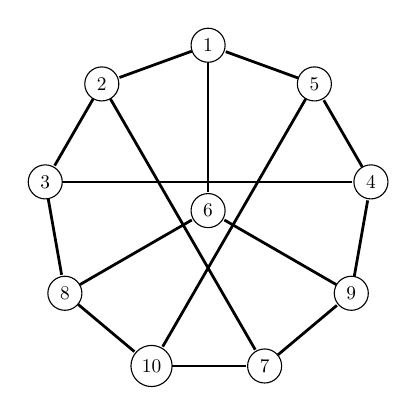
\begin{tikzpicture}[shorten >=0.5pt, auto,
        every node/.style={scale=0.7}, scale=0.7]
        \tikzstyle{nodeStyle} = [circle,draw=black,fill=white]
        \tikzstyle{blackEdge} = [draw=black, line width=1]
        \node[nodeStyle] (1) at (0,0) {6};
        \node[nodeStyle] (2) at (90:3) {1};
        \node[nodeStyle] (3) at (130:3) {2};
        \node[nodeStyle] (4) at (170:3) {3};
        \node[nodeStyle] (5) at (210:3) {8};
        \node[nodeStyle] (6) at (250:3) {10};
        \node[nodeStyle] (7) at (290:3) {7};
        \node[nodeStyle] (8) at (330:3) {9};
        \node[nodeStyle] (9) at (10:3) {4};
        \node[nodeStyle] (10) at (50:3) {5};
        \foreach \from/\to in {2/3,3/4,4/5,5/6,6/7,7/8,8/9,9/10/,10/2,
                               5/1,8/1,2/1,4/9,3/7,10/6}
            \path[blackEdge] (\from) edge (\to);
    \end{tikzpicture}
    \caption{Outra configuração do grafo de Petersen}
\end{figure}

Se tentar procurar um circuito de tamanho menor que 5 no grafo de
Petersen em pouco tempo verá que não está tendo sucesso. Isso sugere que
talvez o menor comprimento de um circuito nesse grafo, sua
\textbf{cintura}, valha 5. De fato, é fácil encontrar um circuito de tamanho 5 na
Figura 3, tome a sequencia $(1,6,9,4,5)$ por exemplo. Dessa forma se
provarmos que a cintura não pode ser menor 5, então está provado que 
$\text{cint}(G)=5$. Uma prova desse fato segue.
\begin{proof}
    Para essa prova, usaremos os conjuntos e as definições apresentadas
    em \textbf{Definição 1}.\newline
    Seja $G$ o grafo de Petersen e seja $C$ um circuito em $G$ de
    comprimento $m$. Suponha por absurdo que $m < 5$. Temos dois casos: 
    \begin{itemize}[label={}]
        \item $m = 3$. Nesse caso, suponha que $C = (u,v,w)$ e sem perda
            de generalidade suponha que $u =
            \{a,b\}$, $v =\{i,j\}$ e $w = \{k,l\}$, com $a,b,i,j,k,l \in
            X$. Como $u,v,w$ são dois a dois vizinhos, então $u,v,w$ são
            dois a dois disjuntos, mas então isso implica que
            $a,b,i,j,k,l$ são todos distintos, mas, por definição
            $|X|=5$, o que é um absurdo.
        \item $m=4$. Nesse caso, suponha que $C = (u,v,w,x)$ e sem perda
            de generalidade suponha que $u =
            \{a,b\}$, $v =\{i,j\}$, $w = \{a,c\}$ e $x = \{i,k\}$. De
            fato, devemos ter $u\cap w \neq \emptyset$ e $v \cap x \neq
            \emptyset $ pois caso contrário seria fomar um circuito de
            tamanho 3, contradizendo a hipotese sobre $m$. Portanto,
            devemos ter $a,b,c,i,j,k$ todos distintos, mas sabemos que
            $|X| = 5$, o que é um absurdo.
    \end{itemize}
\end{proof}

Portanto, temos que $\text{cint}(G) = 5$.\par

Pela Figura 3 fica evidente um  circuito de tamanho 9
$(1,2,3,8,10,7,9,4,5)$. Esse, de fato, é o tamanho de um maior circuinto
em $G$, e portanto temos que a \textbf{circunfêrencia} de $G$ vale 9. Na
seção sobre grafos hamiltonianos, veremos porque a circunferência desse
grafo não pode valer 10.

Outro aspecto interessante desse grafo é que se tomar dois vértices
quaisquer, verá que a distância entre eles é no máximo 2. Em
outras palavras, temos que o \textbf{diâmetro} desse grafo vale 2. Um
pequena prova do fato segue.
\begin{proof}
    Seja $G$ o grafo de Petersen. Seja $u$ um vértice qualquer de $G$.
    Sabemos que $u$ possui apenas  3 vizinhos.\newline
    Sejam $i,j,k$ os 3 vizinhos de $u$. Sabemos que
    $i,j,k$ não são vizinhos, caso contrário, teriamos um circuito de
    comprimento menor que 5, um absurdo, pois $\text{cint}(G)=5$. Além
    do vértice $u$ os vértices
    $i,j,k$ não podem ter vértices vizinhos em comum. Suponha, sem perda
    de generalidade, que os vértices $i$ e $j$ possuem um vértice
    vizinho $w$ em comum, então $(u,i,w,j)$ é um circuito de tamanho
    menor que 5, um absurdo.\newline
    Portanto, juntos, os vértices $i,j,k$ são vizinhos de 6 vértices
    distintos e diferentes de $u$, ou seja, os demais vértices do grafo
    $G$. Portanto $u$ possui um caminho de
    comprimento 1 aos vértices $i,j,k$ e um caminho de comprimento de tamanho 2 aos
    demais vértices do grafo.\newline
    Assim, temos que $\text{diam}(G)=2$.
\end{proof}

Por último, verá que não conseguirá encontrar uma bipartição em $G$.
Isso se deve ao fato de que o grafo de Petersen não é bipartido. Segue
a prova.
\begin{proof}
    Pela \textbf{proposição 1.6} das notas de aula sabemos que um grafo
    é bipartido se e somente se não possui circuitos ímpares. Sabemos
    que $G$ possui um circuito de tamanho 5, pois $\text{cint}(G)=5$.
    Portanto, o grafo de Petersen não pe bipartido.
\end{proof}

\section{Grafos Eulerianos}
Dizemos que um grafo conexo possui um \textbf{trilha euleriana} se ele possui
uma trilha que passa por todas as arestas de um grafo. Se um grafo
conexo
possui uma trilha euleriana fechada, dizemos que ele é um $grafo
euleriano$.\newline
O grafo de Petersen não é Euleriano. Segue a prova:
\begin{proof}
    De acordo com o \textbf{teorema 2.1} um grafo é euleriano se e só se
    todos
    os seus vértices possuem grau par. Todos os vértices do grafo de
    Petersen possuem grau 3, ou seja, grau impar. Portanto o grafo de
    Petersen Euleriano.
\end{proof}

Além disso, o grafo de Petersen também não possui um trilha euleriana.
Segue a prova:
\begin{proof}
    Pelo \textbf{corolário 2.2} sabemos que um grafo possui uma trilha
    euleriano se e só se esse grafo possui no máximo dois vértices de
    grau ímpar. O grafo de Petersen possui 10 vérties de grau ímpar e,
    portanto, não possui uma trilha euleriana.
\end{proof}

De acordo com o \textbf{corolário 2.3} se um grafo $G$ possui $2k>2$
vértices de grau ímpar então é possível particionar $A(G)$ em $k$
trilhas disjuntas nas arestas. O grafo de Petersen possui 10 vértices de
grau ímpar, portanto deve ser possível encontrar 5 trilhas disjuntas nas
arestas que cubram todas as areastas de $G$. Tal configuração de
caminhos pode ser vista na \textbf{Figura 4}, cada caminho foi colorido de
uma cor diferente para faciliar a vizualização.
\begin{figure}[H]
    \centering
    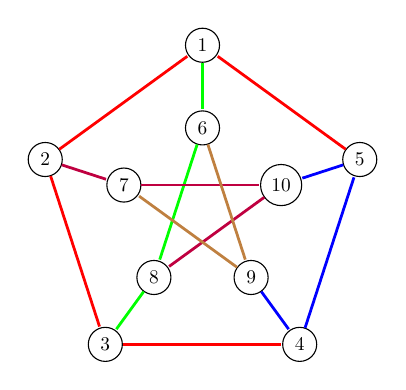
\begin{tikzpicture}[shorten >=0.5pt, auto,
        every node/.style={scale=0.7}, scale=0.7]
        \tikzstyle{nodeStyle} = [circle,draw=black,fill=white]
        \tikzstyle{blackEdge} = [draw=black, line width=1]
        \node[nodeStyle] (6) at (90:1.5) {6};
        \node[nodeStyle] (1) at (90:3) {1};
        \node[nodeStyle] (7) at (162:1.5) {7};
        \node[nodeStyle] (2) at (162:3) {2};
        \node[nodeStyle] (8) at (234:1.5) {8};
        \node[nodeStyle] (3) at (234:3) {3};
        \node[nodeStyle] (9) at (306:1.5) {9};
        \node[nodeStyle] (4) at (306:3) {4};
        \node[nodeStyle] (10) at (378:1.5) {10};
        \node[nodeStyle] (5) at (378:3) {5};
        \foreach \from/\to in {2/1,5/1,2/3, 3/4}
            \path[blackEdge] (\from) edge[color=red] (\to);
        \foreach \from/\to in {9/4, 4/5,5/10}
            \path[blackEdge] (\from) edge[color=blue] (\to);
        \foreach \from/\to in {1/6,6/8,8/3}
            \path[blackEdge] (\from) edge[color=green] (\to);
        \foreach \from/\to in {2/7,7/10,10/8}
            \path[blackEdge] (\from) edge[color=purple] (\to);
        \foreach \from/\to in {6/9, 9/7}
            \path[blackEdge] (\from) edge[color=brown] (\to);
    \end{tikzpicture}
    \caption{Partição das arestas do grafo de Petersen em 5 trilhas
    disjuntas nas arestas}
\end{figure}
    
    Um pergunta interessante a se fazer seria: qual o número de mínimo
    de arestas a serem adicionadas do grafo de Petersen de forma que o
    grafo resultante seja euleriano. Bem, sabemos que todo vértice no
    grafo de Petersen tem grau impar, ou sejam, 10 vértices. Sabemos
    também que cada aresta
    inserida tem o potencial de transformar dois vértices de grau impar
    em vértices de grau par. Isso sugere que o número $k$ mínimo de arestas
    a serem inseridas deve ser $k\geq 10/2 = 5$. Portanto, se
    conseguirmos encontrar 5 arestas que quando inseridas o grafo
    resultante é euleriano então sabemos que esse número mínimo vale 5.
    De fato, conseguimos encontrar tais 5 arestas, interativamente
    acrescentar arestas entre dois vértices de grau impar não viznhos.
    Uma possivel organização  grafo resultante fica como na \textbf{Figura 5}.
\begin{figure}[H]
    \centering
    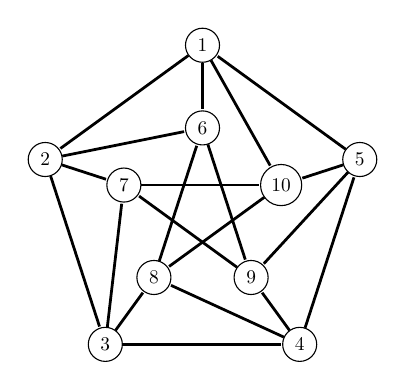
\begin{tikzpicture}[shorten >=0.5pt, auto,
        every node/.style={scale=0.7}, scale=0.7]
        \tikzstyle{nodeStyle} = [circle,draw=black,fill=white]
        \tikzstyle{blackEdge} = [draw=black, line width=1]
        \node[nodeStyle] (6) at (90:1.5) {6};
        \node[nodeStyle] (1) at (90:3) {1};
        \node[nodeStyle] (7) at (162:1.5) {7};
        \node[nodeStyle] (2) at (162:3) {2};
        \node[nodeStyle] (8) at (234:1.5) {8};
        \node[nodeStyle] (3) at (234:3) {3};
        \node[nodeStyle] (9) at (306:1.5) {9};
        \node[nodeStyle] (4) at (306:3) {4};
        \node[nodeStyle] (10) at (378:1.5) {10};
        \node[nodeStyle] (5) at (378:3) {5};
        \foreach \from/\to in {1/2,2/3,3/4,4/5,5/1,
                               1/6, 2/7, 3/8, 4/9, 5/10,
                               7/10, 10/8, 8/6, 6/9, 9/7,
                               2/6, 1/10, 5/9, 4/8, 3/7}
            \path[blackEdge] (\from) edge (\to);
        
    \end{tikzpicture}
    \caption{Grafo euleriano resultante de inserções de arestas no grafo
    de Petersen}
\end{figure}
    Note que todo vértice possui grau par e, portanto, o grafo é euleriano.
\section{Árvores}
Árvores são grafos conexos minimais, ou seja, são grafos conexos com a
menor quantidade de arestas possível. Uma propriedade marcantes desses
grafos é que eles possuem $n-1$, onde $n$ é o número de vértices no
grafo. Claramente o grafo de Petersen não é uma árvore.\newline
Por outro lado, como o grafo de Petersen é conexo, então, pelo
\textbf{corolário 3.6}, ele possui pelo menos uma árvore geradora. De
fato, o grafo de Petersen não possui só uma árvore geradora, mas várias.
Uma árvore genadora de exemplo pode ser vista na \textbf{Figura 5}.
\begin{figure}[H]
    \centering
    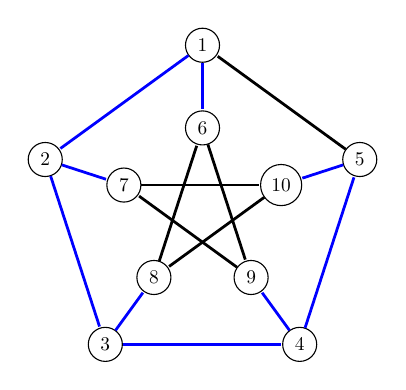
\begin{tikzpicture}[shorten >=0.5pt, auto,
        every node/.style={scale=0.7}, scale=0.7]
        \tikzstyle{nodeStyle} = [circle,draw=black,fill=white]
        \tikzstyle{blackEdge} = [draw=black, line width=1]
        \node[nodeStyle] (6) at (90:1.5) {6};
        \node[nodeStyle] (1) at (90:3) {1};
        \node[nodeStyle] (7) at (162:1.5) {7};
        \node[nodeStyle] (2) at (162:3) {2};
        \node[nodeStyle] (8) at (234:1.5) {8};
        \node[nodeStyle] (3) at (234:3) {3};
        \node[nodeStyle] (9) at (306:1.5) {9};
        \node[nodeStyle] (4) at (306:3) {4};
        \node[nodeStyle] (10) at (378:1.5) {10};
        \node[nodeStyle] (5) at (378:3) {5};
        \foreach \from/\to in {1/2,2/3,3/4,4/5,
                               1/6, 2/7, 3/8, 4/9, 5/10}
            \path[blackEdge] (\from) edge[color=blue] (\to);
        \foreach \from/\to in {5/1,7/10, 10/8, 8/6, 6/9, 9/7}
            \path[blackEdge] (\from) edge (\to);
    \end{tikzpicture}
    \caption{Uma árvore geradora do grafo de Petersen em azul}
\end{figure}
\section{Grafos Hamiltonianos}
Um caminho (ou circuito) hamiltoniano é um caminho (ou circuito) que
passa por todos os vértices de um grafo. Dizemos que um grafo é
hamiltoniano se ele possui um circuito hamiltoniano.\par
Se procurar, verá que o grafo de Petersen possui um caminho
hamiltoniano. Esse caminho é fácil de ver na Figura 3, basta tomar o
seguinte caminho $(2,3,8,10,7,9,4,5,1,6)$.\par
Por outro lado encontrará problemas se tentar encontrar um circuito
hamiltoniano no grafo de Petersen, porque o grafo de Petersen não é
hamiltoniano. Uma prova segue:
\begin{proof}
    Seja $G$ o grafo de Petersen. Suponha, por absurdo, que $G$ é hamiltoniano.
    Então existe um circuito $C = (v_1, \dots, v_{10})$ que passa por
    todos os vértices de $G$.
    \begin{figure}[H]
    \begin{subfigure}{.5\textwidth}
        \centering
        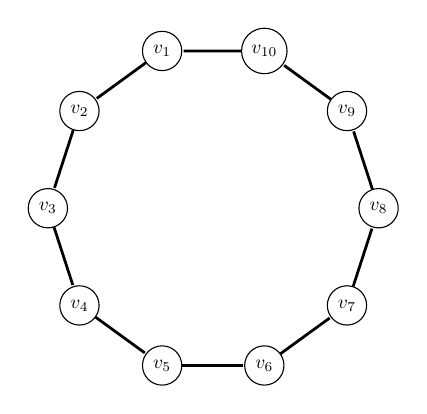
\begin{tikzpicture}[shorten >=0.5pt, auto,
            every node/.style={scale=0.7}, scale=0.7]
            \tikzstyle{nodeStyle} = [circle,draw=black,fill=white]
            \tikzstyle{blackEdge} = [draw=black, line width=1]
            \node[nodeStyle] (1) at (108:3) {$v_1$};
            \node[nodeStyle] (2) at (144:3) {$v_2$};
            \node[nodeStyle] (3) at (180:3) {$v_3$};
            \node[nodeStyle] (4) at (216:3) {$v_4$};
            \node[nodeStyle] (5) at (252:3) {$v_5$};
            \node[nodeStyle] (6) at (288:3) {$v_6$};
            \node[nodeStyle] (7) at (324:3) {$v_7$};
            \node[nodeStyle] (8) at (0:3)   {$v_8$};
            \node[nodeStyle] (9) at (36:3)  {$v_9$};
            \node[nodeStyle] (10) at (72:3) {$v_{10}$};
            \foreach \from/\to in {1/2,2/3,3/4,4/5,5/6,6/7,7/8,8/9,
                                9/10, 10/1}
                \path[blackEdge] (\from) edge (\to);
        \end{tikzpicture}
        \caption{Circuito}
    \end{subfigure}
     \begin{subfigure}{.5\textwidth}
        \centering
        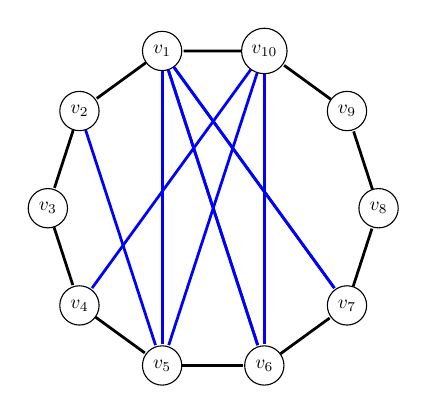
\begin{tikzpicture}[shorten >=0.5pt, auto,
            every node/.style={scale=0.7}, scale=0.7]
            \tikzstyle{nodeStyle} = [circle,draw=black,fill=white]
            \tikzstyle{blackEdge} = [draw=black, line width=1]
            \node[nodeStyle] (1) at (108:3) {$v_1$};
            \node[nodeStyle] (2) at (144:3) {$v_2$};
            \node[nodeStyle] (3) at (180:3) {$v_3$};
            \node[nodeStyle] (4) at (216:3) {$v_4$};
            \node[nodeStyle] (5) at (252:3) {$v_5$};
            \node[nodeStyle] (6) at (288:3) {$v_6$};
            \node[nodeStyle] (7) at (324:3) {$v_7$};
            \node[nodeStyle] (8) at (0:3)   {$v_8$};
            \node[nodeStyle] (9) at (36:3)  {$v_9$};
            \node[nodeStyle] (10) at (72:3) {$v_{10}$};
            \foreach \from/\to in {1/2,2/3,3/4,4/5,5/6,6/7,7/8,8/9,
                                   9/10, 10/1}
                \path[blackEdge] (\from) edge (\to);
            \foreach \from/\to in {1/5,1/6,1/7}
                \path[blackEdge] (\from) edge[color=blue] (\to);
            \foreach \from/\to in {10/4,10/5,10/6}
                \path[blackEdge] (\from) edge[color=blue] (\to);
            \foreach \from/\to in {2/5,1/6,1/7}
                \path[blackEdge] (\from) edge[color=blue] (\to);
        \end{tikzpicture}
        \caption{Circuito}
    \end{subfigure}
        \caption{Provade que o grafo de Petersen não é Hamiltoniano}
\end{figure}
\end{proof}
\end{document}
